\documentclass[Japanese]{dicomopapers}
%\documentclass[Japanese,noauthor]{dicomopapers}

\usepackage[dvips]{graphicx}
\usepackage{latexsym}

\def\Underline{\setbox0\hbox\bgroup\let\\\endUnderline}
\def\endUnderline{\vphantom{y}\egroup\smash{\underline{\box0}}\\}
\def\|{\verb|}

\begin{document}

% 和文表題
\title{IoTデバイスの通信セキュリティ向上のための\\ホームネットワーク仮想化フレームワークの提案}
% 英文表題
\etitle{Proposal of Home Network Virtualization Framework\\to Improve Communication Security of IoT Devices}

% 所属ラベルの定義
\affiliate{DOSHISHA}{同志社大学大学院 理工学研究科\\Graduate School of Science and Engineering, Doshisha University}
\affiliate{MOBILITY}{同志社大学モビリティ研究センター\\Mobility Reserch Center, Doshisha University}

\author{塚崎 拓真}{TAKUMA TSUKASAKI}{DOSHISHA}
\author{滕 睿}{RUI TENG}{MOBILITY}
\author{佐藤 健哉}{KENYA SATO}{DOSHISHA}

\begin{abstract}
	近年,IoT(Internet of Things)が注目を集めるようになり,今後あらゆるモノがネットワークに接続され,利用されることが予想される.しかし,IoTの発展により利便性が高まる一方で,これまでネットワークに接続されていなかったモノが接続されることにより,セキュリティ上のリスクも高まっている.IoTデバイスは十分なセキュリティを考慮せずに開発されたものが多いため,悪意のある攻撃者によるサイバー攻撃の標的になりやすい.また,現在のスマートホームデバイスは,クラウド上のシステムと連携することで,デバイス間の連携を可能にしているが,今後はホームネットワーク内で閉じたデバイス間の通信によって連携を行う形になることが想定される.デバイス間で直接通信を行う場合,各デバイスにおいてどのデバイスとの通信を受け入れるか,アクセス制御を行う必要がある.しかし,IoTデバイスは従来のPC等の既存機器と比較した場合,CPU等のリソースを十分に保持していないため,デバイスの計算能力の制限やソフトウェア自体の脆弱性によって,適用できる機能が限られるという問題がある.そのため,ホームネットワーク内で通信するのであれば,どのデバイスも必ず利用するネットワークを利用したシステムを構築することが望ましい.そこで本研究では,SDN(Software Defined Networks)の代表的プロトコルであるOpenFlowを用いて,ホームネットワーク内の通信を監視するフレームワークの構築を検討した.提案システムでは,セキュリティ対策を適用可能なデバイスをProxyと定義し,ルータ上に仮想的に作成する.ここに,IoTデバイスがリソース量の制限により適用できないセキュリティ対策をオフロードし,このProxyがIoTデバイス間の通信を中継することで,本来IoTデバイスに適用したいセキュリティ対策を実現する.セキュリティ対策として,ホームネットワーク内の通信のトラフィック情報は既知であることを考慮し,フローの検証をOpenFlowコントローラで行う.ルータ内にコンテナを配置し,そのコンテナ上にProxyを作成する.そして,IoTデバイス間で閉じた通信を行うシミュレーションの評価を行い,ホームネットワークにおいてセキュリティ要件を保つことを示した.

\end{abstract}

% 表題などの出力
\maketitle

% 本文はここから始まる
\section{はじめに}
近年,IoT(Internet of Things)が注目を集めるようになり,今後あらゆるモノがネットワークに接続され,利用されることが予想される.\par
しかし,IoTの発展により利便性が高まる一方で,これまでネットワークに接続されていなかったモノが接続されることにより,セキュリティ上のリスクも高まっている\cite{guideline}.
IoTデバイスは十分なセキュリティを考慮せずに開発されたものが多いため,悪意のある攻撃者によるサイバー攻撃の標的になりやすい.
また,現在のスマートホームデバイスは,クラウド上のシステムと連携することで,デバイス間の連携を可能にしているが,今後はホームネットワーク内で閉じたデバイス間の通信によって連携を行う形になることが想定される.
デバイス間で直接通信を行う場合,各デバイスにおいてどのデバイスとの通信を受け入れるか,アクセス制御を行う必要がある.
% セキュリティ上の脅威が各種デバイスに顕在した場合,個別に対処するとコストや時間がかかってしまうため,脅威に対し一括に対処する必要がある.\par
% しかし,ホームネットワーク内には異なる規格のハードウェアや様々なアプリケーションが混在しているため,それら全てに対応したシステムの構築や更新を続けるのは困難である.
% しかし,全てのデバイスがアクセス制御に対応しているとは限らず,デバイスの計算能力の制限によって実現できるアクセス制御に制限がある場合や,デバイスのソフトウェア自体の脆弱性によってアクセス制御が機能しない場合が考えられる.
しかし,IoTデバイスは従来のPC等の既存機器と比較した場合,CPU等のリソースを十分に保持していないため,デバイスの計算能力の制限やソフトウェア自体の脆弱性によって,適用できる機能が限られるという問題がある.
そのため,ホームネットワーク内で通信するのであれば,どのデバイスも必ず利用するネットワークを利用したシステムを構築することが望ましい.\par
そこで本研究では,SDN(Software Defined Networks)の代表的プロトコルであるOpenFlowを用いて,ホームネットワーク内の通信を監視するフレームワークの構築を検討した.
% OpenFlowを利用することで,既存IoTデバイスや異なる規格などに対応でき,ホームネットワークに適した形で不正な通信の検知を実現する.
提案システムでは,セキュリティ対策を適用可能なデバイスをProxyと定義し,ルータ上に仮想的に作成する.
ここに,IoTデバイスがリソース量の制限により適用できないセキュリティ対策をオフロードし,このProxyがIoTデバイス間の通信を中継することで,本来IoTデバイスに適用したいセキュリティ対策を実現する.
セキュリティ対策として,ホームネットワーク内の通信のトラフィック情報は既知であることを考慮し,フローの検証をOpenFlowコントローラで行う.\par
ルータ内にコンテナを配置し,そのコンテナ上にProxyを作成する.そして,IoTデバイス間で閉じた通信を行うシミュレーションの評価を行い,ホームネットワークにおいてセキュリティ要件を保つことを示した.

\begin{figure}[!tb]
	\centering
	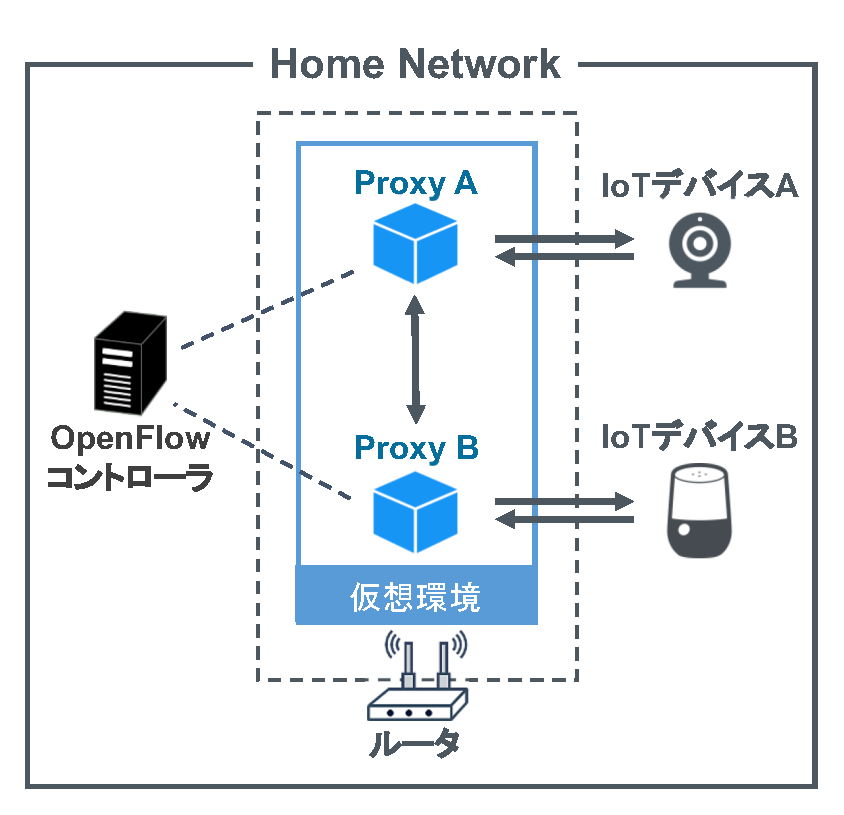
\includegraphics[width=\linewidth]{img/system.eps}
	\caption{提案システムの構成}
	\label{fig:system}
\end{figure}

\section{関連研究}

\section{提案システム}
\subsection{概要}
提案システムでは,セキュリティ対策を適用可能なデバイスをProxyと定義し,ルータ上に仮想的に作成する.
ここに,IoTデバイスがリソース量の制限により適用できないセキュリティ対策をオフロードし,このProxyがIoTデバイス間の通信を中継することで,本来IoTデバイスに適用したいセキュリティ対策を実現する.
セキュリティ対策として,ホームネットワーク内の通信のトラフィック情報は既知であることを考慮し,フローの検証をOpenFlowコントローラで行う.

\subsection{システム構成}
提案システムの構成を\figref{fig:system}に示す.本提案システムの構成要素は,IoTデバイス,Proxy,ルータ,仮想環境から構成される.
\begin{itemize}
	\item \underline{IoTデバイス}\mbox{}\\
	      本研究で扱うIoTデバイスは,センサーをはじめとした,CPU等のリソースを十分に保持しておらず,直接セキュリティ対策を適用できないデバイスと定義する.
	\item \underline{Proxy}\mbox{}\\
	      IoTデバイスに要求されるセキュリティ対策を,仮想的に実現したものである.IoTデバイスからの通信を中継し,セキュリティ対策を適用する.セキュリティ対策ごとに作成し,IoTデバイスと紐づけることで,対象デバイスに応じた必要な対策を実現できる.
	\item \underline{ルータ}\mbox{}\\
	\item \underline{仮想環境}\mbox{}\\
	      Proxyの実行環境である.Proxyが作成される際に要求されるリソースを十分に提供することが可能である.
\end{itemize}

\section{実装}
\subsection{実装環境}
本研究の実装環境、実装環境の構成をそれぞれに示す.Proxyの作成方法としては軽量なアプリケーション実行環境であるDockerを利用した.ProxyをDockerで作成されるコンテナ状で稼働させることで複数の論理デバイスをリソース、オーバーヘッドを抑えて作成できることに加え、Docker Hubより配布されるDocker Imageを用いることで容易に作成可能となる.また今回扱う通信プロトコルとしてはhttp(REST)を想定する.

\subsection{動作手順}

\subsection{想定ユースケース}
本提案システムを用いた想定ユースケースを以下に示す.各DockerイメージはDocker Hubというユーザが作成したコンテナをアップロードして公開・共有できるサービスを利用することを想定する.

\begin{itemize}
	\item \underline{リソースを使うセキュリティ対策をあらかじめ提供する場合}\mbox{}\\
	      SSLによる通信の暗号化など、IoTデバイスのリソースを多く利用するために適用できないセキュリティ対策をあらかじめDockerイメージとして提供し、論理デバイス上で実現する.
	\item \underline{インシデント発生時などに対策を提供する場合}\mbox{}\\
	      事前に提供していたセキュリティ対策では想定していなかったインシデント等が発生した場合等に、当該デバイスの持つリソース量に依存せず、追加のセキュリティ対策を提供することが可能となる.
\end{itemize}

\section{評価}
\subsection{評価内容}

\subsection{評価環境}

\section{結果と考察}
\subsection{評価結果}

\subsection{性能に関する考察}

\subsection{信頼性に関する考察}
IoTデバイスを用いたシステムの安心安全を確保するための機能として,IPAによりIoT高信頼化昨日が定義されており,IoT高信頼化要件として,IPAによりIoT高信頼化要件として,開始,予防,検知,回復,終了の5つの局面に分けてそれぞれセキュリティ要件が定義されている\cite{IPA}.今回は前述の5つより,システム稼働中の局面である予防,検知,回復の3つにおける高信頼化要件に対し,提案システムの有効性について考察する.

\begin{itemize}
	\item \underline{予防の局面における考察}\mbox{}\\
	      予防の局面での高信頼化要件は,稼働中の異常発生を未然に防止できることである.これに対応するIoT高信頼化機能としては,ログ取集機能,暗号化機能等があり,以上の予兆の把握,資産の保護を実現する.提案システムを用いることで,リソース量の関係で通常のIoTデバイスに適用できない機能であっても適用可能となる.
	\item \underline{検知の局面における考察}\mbox{}\\
	      検知の局面での高信頼化要件は,稼働中の異常発生を早期に検知できることである.これに対応するIoT高信頼化機能としては,状態監視機能,ログ収集機能があり,以上発生の検知や発生原因の特定を実現する.提案システムを用いることで,予防の局面同様,デバイスのリソース量に依存せず,求められる機能を実現できることに加え,Proxyは書くIoTデバイスごとに作成するため,個々のデバイスに応じた詳細な検知ルールを適用可能となる.
	\item \underline{回復の局面における考察}\mbox{}\\
	      回復の局面での高信頼化要件は,異常が発生した場合に稼働の復旧ができることである.特にIoTでは,さまざまなデバイスが相互通信を行うため,事前に予測していなかった異常が発生することが考えられる.今回の環境では各セキュリティ対策はDocker Hubを通してDockerイメージとして提供することで,事前に作成したセキュリティ対策だけでなく,追加のセキュリティ対策も配布・適用が容易である.
\end{itemize}

\section{まとめ}

\begin{thebibliography}{10}
	\bibitem{guideline} IoT推進コンソーシアム, 総務省, 経済産業省, "IoTセキュリティガイドライン ver 1.0", 2016.
	\bibitem{d2d} C. Vallati et al., "Mobile-Edge Computing Come Home Connecting things in future smart homes using LTE device-to-device communications", IEEE Consumer Electronics Magazine, Vol.5, No.4, pp.77-83, 2016.
	\bibitem{disap} M. Serror et al., "Towards In-Network Security for Smart Homes", Proceedings of the 13th International Conference on Availability, Reliability and Security (ARES 2018), No.18, pp.1-8, 2018.
	\bibitem{OpenFlow} Nick McKeown et al., "OpenFlow: enabling innovation in campus networks", SIGCOMM Computer Communication Review, Vol.38, pp. 69–74, 2008.
	\bibitem{IPA} IPA技術本部 ソフトウェア高信頼化センター(SEC), "「つながる世界の開発指針」の実践に向けた手引き", 2017.
	\bibitem{webpage}
	情報処理学会: 情報処理学会論文誌(IPSJ Journal)原稿執筆案内,情報処理学
	会(オンライン),
	\urlj{https://\\www.ipsj.or.jp/journal/submit/ronbun\_j\_prms.html}
	\refdatej{2022-03-01}.
\end{thebibliography}

\end{document}
